\documentclass[11pt]{article}
\usepackage{graphicx}
\usepackage{hyperref}
\usepackage{placeins}

\title{{Gouda Turtle Dictionary} \\ User Manual}
\date{}

\begin{document}
\maketitle

\section{Forward}
Gouda Turtle Dictionary is a lightweight in-browser word lookup extension for
Mozilla Firefox. It provides a tool to look up words quickly and easily.
When the application is invoked
it displays the definitions from the primary word resource
and provides links to other word resources.
Additionally, it stores the words that have been looked up by the user and
provides the user with a \textit{Word of the Day}, a periodic pop-up
reminding the user of words he or she has looked up previously.
The \textit{Word of the Day}
can be disabled.

\section{Installing the Application}
The application is hosted at
\href{http://gtdict.cslabs.clarkson.edu/}{http://gtdict.cslabs.clarkson.edu/}.
Install the application by clicking the appropriate link and following the
on-screen instructions.

\section{Using the Application}
\subsection{Define Words}
To define an unknown word, follow the steps listed below.

\begin{enumerate}
\item{Make sure the extension is installed}
\item{Highlight a word to be looked up}
\item{Right-click anywhere on the web page and select `GT Dictionary' from the
context menu, or key in the configured hotkey combination}
\end{enumerate}

\begin{figure}[ht!]
\centering
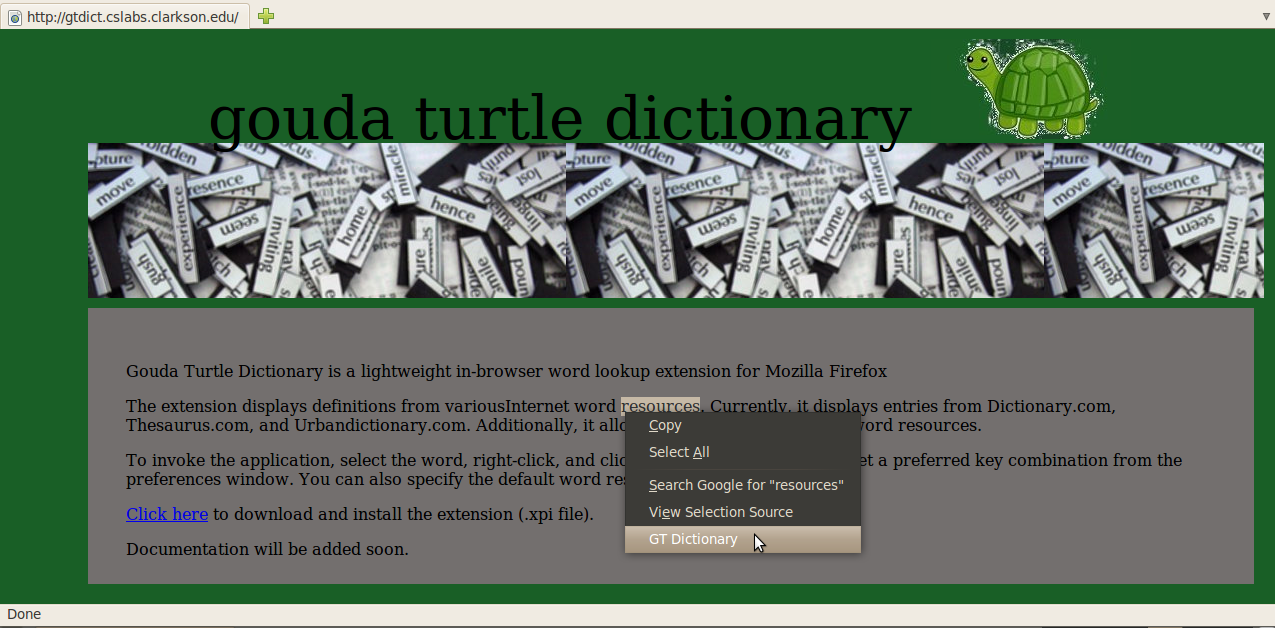
\includegraphics[scale=0.30]{gt0.png}
\caption{GT Dictionary Context Menu Item}
\label{right}
\end{figure}

%% Have we tested this recently?
%If you are on a Mac, the default key combination is OPTION+SHIFT+K.
Invoking the application will bring up the `GT Dictionary' window.
This contains the definition of the word from your primary word resource, as
well as buttons that open links to entries from other word
resources. Available buttons are listed below.
\begin{itemize}
\item{\url{http://dictionary.com/}}
\item{\url{http://thesaurus.com/}}
\item{\url{http://www.urbandictionary.com/}}
\item{\url{http://en.wikipedia.org/wiki/Wiki}}
\end{itemize}
Error messages will be displayed if a word is not highlighted or if an entry is
not found. If this occurs, the buttons will link to the home page of the word
resource.

\subsection{Word of the Day}
The \textit{Word of the Day} functionality stores the words looked up by the user.
After the time interval specified in the preferences
has passed, the next time a new Firefox window is opened,
the \textit{Word of the Day} window launches.
It contains a word and its entry from the default word resource.
If the \textit{Word of the Day} is deactivated,
it will not store or display words.

\section{Customization}
To launch the preferences window, follow the instructions below:

\begin{enumerate}
    \item{In your Firefox window, go to
    \emph{Tools} $\rightarrow$ \emph{Add-ons}}
    \item{Find \emph{Gouda Turtle Dictionary} and click on \emph{Preferences}.}
\end{enumerate}

\begin{figure}[ht!]
\centering
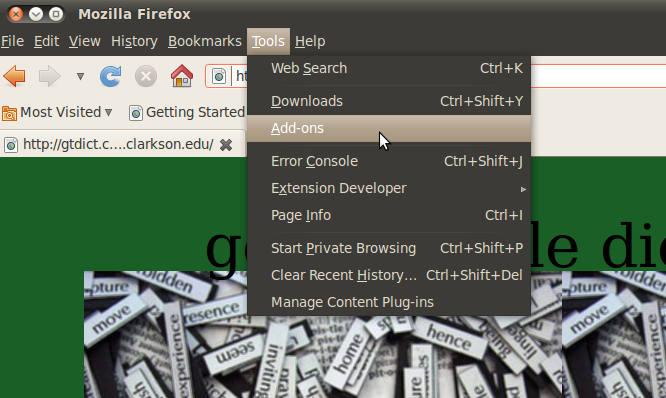
\includegraphics[scale=0.3]{gt2.png}
\caption{Finding the Add-ons Menu}
\label{prefs}
\end{figure}

Once in the preferences window, one can customize the hotkey, default word
resource, toggle \textit{Word of the Day} on and off, and specify the
frequency at which \textit{Word of the Day} produces pop-up windows.

\begin{figure}[ht!]
\centering
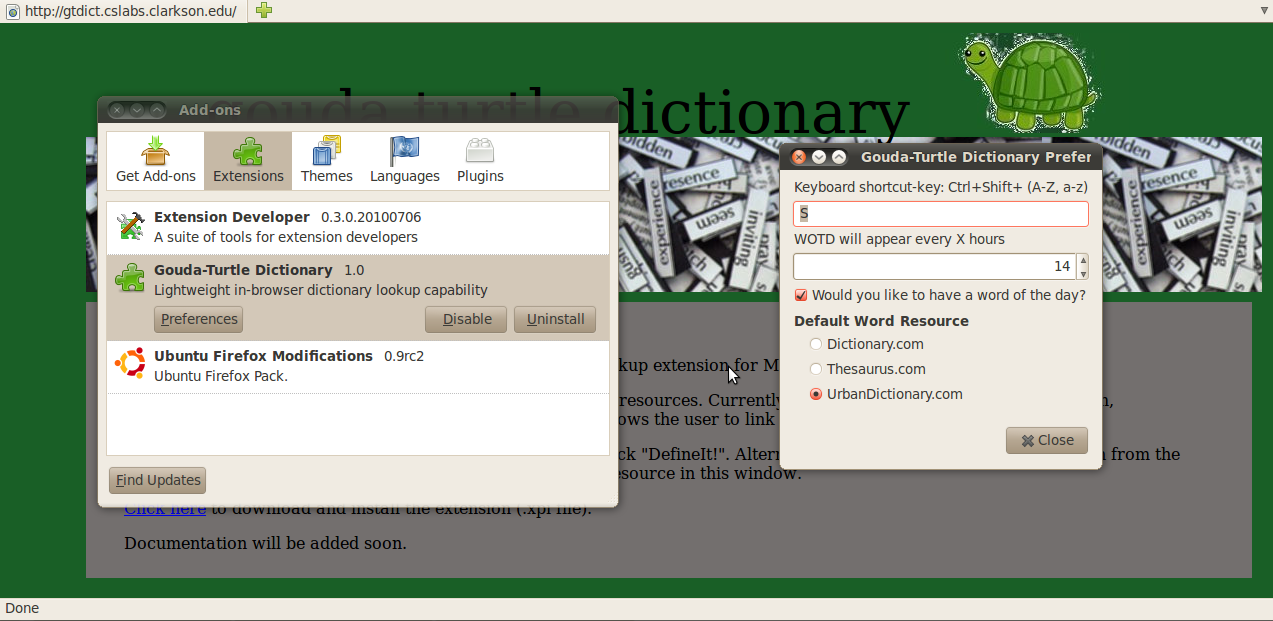
\includegraphics[scale=0.3]{gt1.png}
\caption{Preferences Pane}
\label{gtfoo}
\end{figure}

\FloatBarrier
Specify a keyboard shortcut key \textit{k},
where CTRL+SHIFT+\textit{k} would invoke the ``GT Dictionary'' window.
The default shortcut key is the letter  \emph{K}.
Avoid key combinations that are already mapped to different functionalities by
the operating system, Firefox, or other extensions.
Select the time interval (in hours) you would like to wait between receiving
new \textit{Word of the Day} pop-ups. Use the check-box to activate/deactivate
the \textit{Word of the Day} feature.

Use the radio boxes to select the default word resource.
The default word resource is \url{http://urbandictionary.com/}.
The options include:
\begin{itemize}
\item{\url{http://dictionary.com/}}
\item{\url{http://thesaurus.com/}}
\item{\url{http://www.urbandictionary.com/}}
\end{itemize}


When finished customizing the application, simply close the preferences window.
\end{document}
